\section{Анализ требований к программному средству и разработка функциональных требований}
\label{sec:domain}

\subsection{Функциональная модель программного средства}
\label{sec:domain:model}

Функциональная модель программного средства представлена в виде\linebreakсхемы алгоритма процесса слежения за персональными расходами и диаграммы вариантов использования и информационной модели предметной области. Варианты использования отражают функциональность системы в ответ на внешние воздействия с точки зрения получения значимого результата для пользователей. Информационная модель предметной области в дальнейшем будет использоваться при проектировании базы данных для программного средства.

\subsubsection{} Анализ процесса слежения за финансами
\label{sec:domain:model:deeds}

Перед началом проектирования необходимо проанализировать процесс слежения за финансами. Результат анализа представлен в виде схемы алгорима на рисунке.

Одной из особенностей схемы является цикличность. Цикл начинается вопросом бота о том, какую команду хотел бы выполнить пользователь. После ввода команды приложение инициализирует диалог, соответствующий заданной команде. После полного выполнения команды, пользователю снова задается вопрос, какую команду он хотел бы выполнить.

Такм образом, на схеме алгоритма приведен вариант процесса слежения за финансами, в который входят задание категорий, изменение категорий, удаление категорий, добавление операций в категорию, а также просмотр статистики. Программное средство направлено на максимальное упрощение ведения пользователькой бухгалтерии.

\subsubsection{} Варианты использования программного средства
\label{sec:domain:model:use_cases}

По результатам анализа предметной области и существующих аналогов можно сделать вывод, что проектируемое программное средство должно поддерживать ряд функций для снижения временных затрат пользователя на ведение своей бухгалтерии, ключевыми из которых являются следующие:

\begin{itemize}
	\item \emph{Добавление категорий}. На категориях строится вся работа с приложением. Пользователь может добавить несколько категорий для более грамотного отслеживания своих финансов.
	\item \emph{Выбор валюты категории}. Валюта категории обеспечивает гибкость в ведении домашней бухгалтерии, так как охватывает больше возможных вариантов использования, будь то расходы на отпуск, либо другие расходы в иностранной валюте.
	\item \emph{Выбор имени категории}.
	\item \emph{Выбор типа категории}. Категории могут быть либо доходами, либо расходами.
	\item \emph{Добавление операций}. Пользователь может добавить операцию по любой категории. 
	\item \emph{Просмотр статистики} по всем категориям, а также по каждой из категорий более детально.
\end{itemize}

Use case диаграмма, разработанная с использованием нотации \uml, представлена на рисунке~\ref{fig:domain:model:use_cases:model}.

\begin{figure}[!h]
\centering
	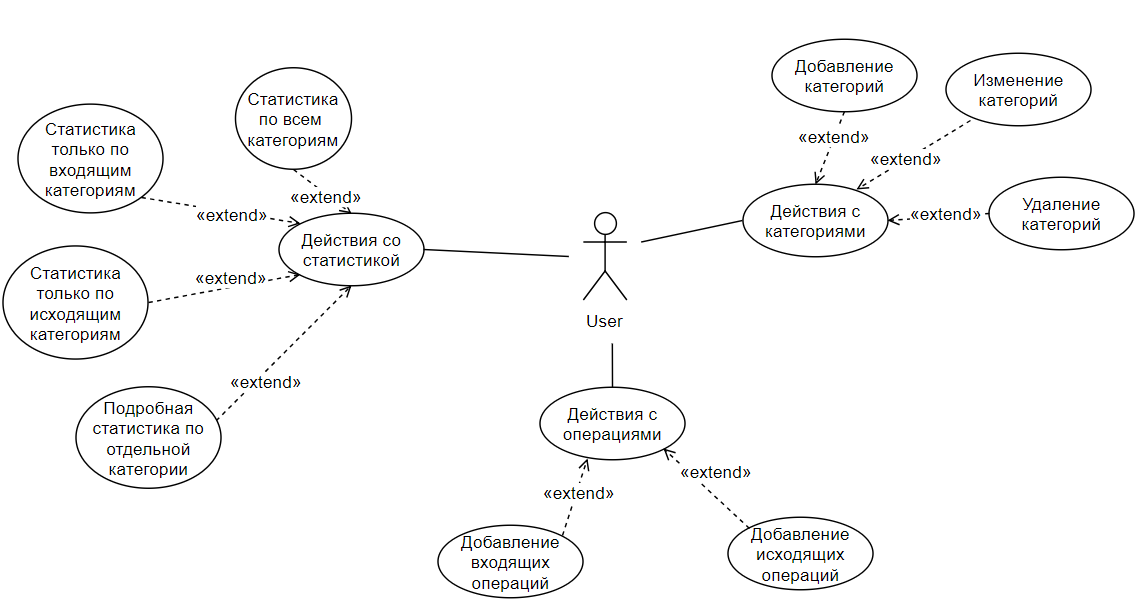
\includegraphics[scale=0.5]{use_case.png}
	\caption{Use case диаграмма ПС}
	\label{fig:domain:model:use_cases:model}
\end{figure}

Рассмотрим подробно представленные на рисунке прецеденты.

\emph{Добавление категорий} -- функция, с помощью которой пользователь может добавить категорию, а также настроить ее по своему усмотрению. После вызова функции добавления категории, должен начаться диалог, в котором приложение последовательно будет задавать вопросы по каждому из пунктов настройки категории. Во время диалога пользователь может вызвать команду отмены. Для завершения диалога настройки, пользователь должен указать тип категории, имя категории, а также валюту. Для категорий расходов пользователь также должен указать желаемый порог расходов.

\emph{Изменение категорий} происходит по такому же сценарию, как и в случае создания. При вызове функции пользователь должен выбрать категорию для изменения. Далее начинается диалог изменения.

Для \emph{удаления категорий} пользователь должен выбрать категорию для удаления.

\emph{Добавление входящих операций} -- функция, с помощью которой пользователь может добавить операцию в одну из категорий-доходов. После вызова функции пользователь должен выбрать категорию для добавления операции. Далее приложение инициализирует диалог добавления операции. Пользователь может отменить создание операции с помощью команды отмены. Для добавления операции в категорию-доход пользователю требуется ввести сумму в валюте категории, а также указать дату. Пользователь может ввести дату вручную, либо нажать кнопку <<now>>.

\emph{Добавление исходящих операций} -- функция, с помощью которой пользователь может добавить операцию в одну из категорий-расходов. Функция отличается от функции добавления входящих операций тем, что после ввода суммы в валюте категории, приложение уведомляет пользователя о скором достижении установленного порога расходов.

Функция \emph{просмотра статистики по всем категориям} позволяет пользователю просматривать статистику доходов и расходов по всему списку категорий. В этом случае на выход пользователю будет предоставлен список из названия категории, а также сумма операций со знаком плюс для категорий-доходов и со знаком минус для категорий-расходов.

Функция \emph{просмотра статистики по входящим категориям} идентична предыдущей, за исключением того, что она предоставляет только список категорий доходов, без категорий-расходов.

Функция \emph{просмотра статистики по исходящим категориям} идентична предыдущей, за исключением того, что она предоставляет только список категорий расходов, без категорий-доходов.

Подробная статистика со всеми операциями предоставляется пользователю функцией \emph{просмотра подробной статистики отдельной категории}. При вызове функции пользователь получает список операций, добавленных в эту категорию, вместе с суммой по операции, а также датой добавления.

\subsubsection{} Разработка инфологической модели базы данных
\label{sec:domain:model:db}

Исходя из необходимости использования в проектируемом приложении базы данных, разработаем ее инфологическую модель. Для ее создания будем использовать расширение диаграммы классов \uml, предназначенное для моделирования баз данных. Полученная диаграмма (рисунок~\ref{fig:domain:model:db:model}) будет являться моделью базы данных инфологического уровня~\cite{kulikov_db_workbook}.

\begin{sidewaysfigure}
\centering
	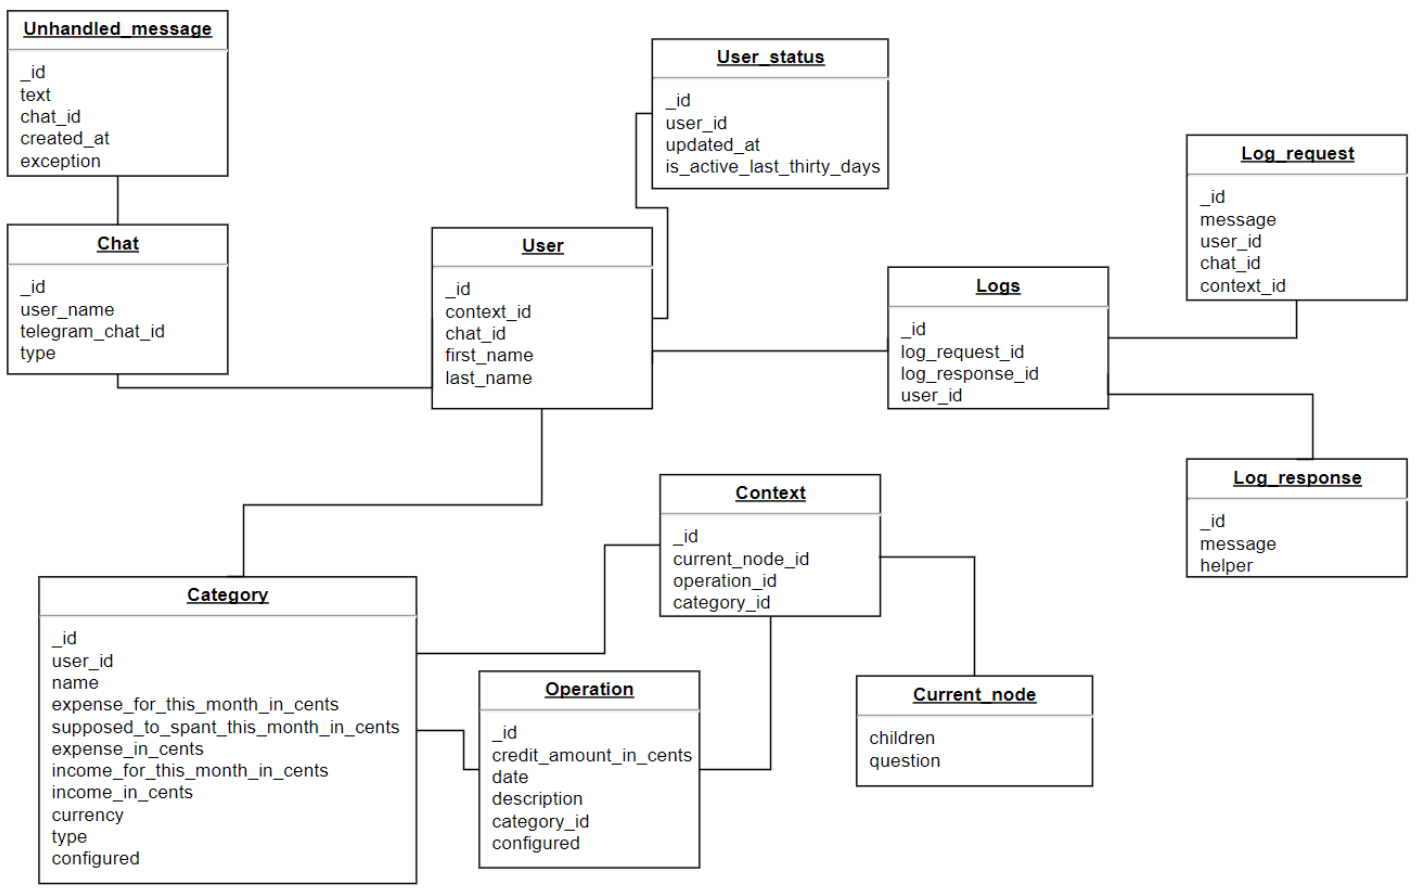
\includegraphics[scale=0.65]{db_schema.png}
	\caption{Инфологическая модель базы данных}
	\label{fig:domain:model:db:model}
\end{sidewaysfigure}

Схема базы данных построена на существующей модели, использующейся на платформе Telegram Bots.

В силу того, что для платформы Telegram Bots не нужно дополнотельно авторизовываться, в таблице \emph{User} отсуствует поле для хешированного пароля. Также, сущность пользователя хранит в себе так называемый контекст пользователя. Контекст требуется для сохранения состояния диалога между пользователем и ботом во время настройки категорий и добавления операций, а также просмотра статистики. 

Сущность \emph{Unhandled message} используется для хранения сообщений об ошибках пользователей, связанных с неправильно обработанными командами, полученными ботом.

Сущность \emph{Chat} хранит в себе информацию о чате между ботом и пользователем, а также его состояние.

Сущность \emph{Category} хранит в себе информацию о категории, включая суммы по доходам/расходам за текущий месяц, а также за все время. Поле \emph{configured} отвечает за состояние конфигурации категории. Если категория не сконфигурирована и пользователь отправляет боту команду отмены, категория удаляется из базы данных.

Сущность \emph{Operation} хранит в себе информацию о конкретной операции, включая сумму, дату добавления и описание. Поле \emph{configured} отвечает за состояние конфигурации операции. Если операция не сконфигурирована и пользователь отправляет боту команду отмены, операция удаляется из базы данных.

Сущность \emph{Context} хранит в себе информацию о текущем контекте диалога между пользователем и ботом. Представляет собой древовидную структуру, с помощью которой бот узнает о том, на какой вопрос пришел ответ от пользователя.

Помимо всего прочего, в схеме базы данных имеются сущности, использующиеся для логирования запросов пользователя и ответов бота. За это отвечают сущности \emph{Log request} и \emph{Log response}. При неправильной работе бота довольно легко обнаружить проблему, используя данные этих сущностей.

\subsection{Разработка спецификации функциональных требований}
\label{sec:domain:specification}

С учетом требований, определенных в подразделе \ref{sec:analysis:specification}, представим детализацию функций проектируемого ПС.

\\[5cm]
\subsubsection{} Функция старта диалога бота
\label{sec:domain:specification:startdialog}

Функция старта диалога бота должна быть реализована с учетом следующих требований:

\begin{enumerate}
	\item После команды \emph{start} в диалоге бота, должна произойти проверка на существование пользователя в базе данных.
	\item В случае отсутствия пользователя в базе, пользователь должен быть создан и добавлен в базу с двумя стандартными категориями, одной для доходов, второй для расходов, а также с обнуленным контекстом пользователя.
	\item Далее должен быть показан список функций бота.
\end{enumerate}

\subsubsection{} Функция добавления категории
\label{sec:domain:specification:addcategory}

Функция добавления категории должна быть реализована с учетом следующих требований:

\begin{enumerate}
	\item Процесс добавления категории инициализируется пользователем бота.
	\item После инициализации процесса бот должен инициализировать контекст пользователя и начать диалог с пользователем для настройки категории.
	\item Для успешной настройки категории, пользователь должен указать тип категории, валюту, название категории, а также желаемый порог расходов для исходящих категорий.
	\item Должна быть реализована обработка неправильных, либо не подходящих по контексту команд. Если такая команда попадает на обработку, пользователю должно быть отправлено сообщение о том, что команда не может быть обработана.
	\item При команде отмена от пользователя, контекст пользователя должен быть очищен, а вновь созданная категория должна быть удалена из базы. После очистки, пользователю должен быть показан список функций бота.
	\item При успешном добавлении категории, контекст пользователя должен быть очищен, вновь созданная категория должна быть переведена в состояние \emph{configured}. Пользователю должен быть показан список функций бота.
\end{enumerate}

\subsubsection{} Функция изменения категории
\label{sec:domain:specification:editcategory}

Функция изменения категории должна быть реализована с учетом следующих требований:

\begin{enumerate}
	\item Процесс изменения категории инициализируется пользователем бота.
	\item После инициализации процесса бот должен инициализировать контекст пользователя и начать диалог с пользователем для настройки категории.
	\item Пользователь должен выбрать, какую категорию он хотел бы изменить.
	\item После выбора категории, пользователь должен перейти к настройке категории, аналогично функции создания.
	\item Для успешной настройки категории, пользователь должен указать тип категории, валюту, название категории, а также желаемый порог расходов для исходящих категорий.
	\item Должна быть реализована обработка неправильных, либо не подходящих по контексту команд. Если такая команда попадает на обработку, пользователю должно быть отправлено сообщение о том, что команда не может быть обработана.
	\item При команде отмена от пользователя, категория должна быть сохранена в состоянии, в котором ее успел изменить пользователь. Контекст пользователя должен быть очищен, а также должен быть показан список функций бота.
	\item При успешном изменени категории, контекст пользователя должен быть очищен, категория должна быть сохранена. Пользователю должен быть показан список функций бота.
\end{enumerate}

\subsubsection{} Функция удаления категории
\label{sec:domain:specification:deletecategory}

Функция удаления категории должна быть реализована с учетом следующих требований:

\begin{enumerate}
	\item Процесс удаления категории инициализируется пользователем бота.
	\item После инициализации процесса бот должен инициализировать контекст пользователя и начать диалог с пользователем для удаления категории.
	\item Пользователь должен выбрать, какую категорию он хотел бы удалить.
	\item Должна быть реализована обработка неправильных, либо не подходящих по контексту команд. Если такая команда попадает на обработку, пользователю должно быть отправлено сообщение о том, что команда не может быть обработана.
	\item После выбора категории, она должна быть удалена, контекст пользователя должен быть очищен, пользователю должен быть показан список функций бота.
	\item При команде отмена от пользователя, контекст пользователя должен быть очищен, а также должен быть показан список функций бота.
\end{enumerate}

\subsubsection{} Функция добавления операции в категорию
\label{sec:domain:specification:addoperationtocategory}

Функция добавления операции в категорию должна быть реализована с учетом следующих требований:

\begin{enumerate}
	\item Процесс добавления операции в категорию инициализируется пользователем бота.
	\item После инициализации процесса бот должен инициализировать контекст пользователя и начать диалог с пользователем для добавления операции.
	\item Пользователь должен выбрать, в какую категорию он хочет добавить операцию.
	\item После выбора категории, пользователь должен перейти к настройке операции.
	\item Должна быть реализована обработка неправильных, либо не подходящих по контексту команд. Если такая команда попадает на обработку, пользователю должно быть отправлено сообщение о том, что команда не может быть обработана.
	\item Для успешной настройки операции, пользователь должен указать сумму операции, а также дату операции.
	\begin{enumerate}
		\item Пользователь может ввести дату вручную в определенном формате.
		\item При желании, пользователь может воспользовать кнопкой <<now>>. В таком случае, операции будет присвоена текущие дата и время.
	\end{enumerate}
	\item При команде отмена от пользователя, контекст пользователя должен быть очищен, а вновь созданная операция должна быть удалена из базы. После очистки, пользователю должен быть показан список функций бота.
	\item При добавлении операции в категорию-расход, если пользователь превысил или близок к тому, чтобы превысить порог, настроенный для категории, должно быть отправлено соответствующее сообщение.
	\item При успешном добавлении операции в категорию, контекст пользователя должен быть очищен, вновь созданная операция должна быть переведена в состояние \emph{configured}. Пользователю должен быть показан список функций бота.
\end{enumerate}

\subsubsection{} Функция просмотра статистики для всех категорий
\label{sec:domain:specification:showallstats}

Функция просмотра статистики для всех категорий должна быть реализована с учетом следующих требований:

\begin{enumerate}
	\item Процесс просмотра статистики для всех категорий инициализируется пользователем бота.
	\item После инициализации процесса бот должен показать пользователю список категорий с суммами их операций.
	\begin{enumerate}
		\item Если категория является категорией-доходом, сумма должна быть отображена со знаком плюс.
		\item Если категория является категорией-расходом, сумма должна быть отображена со знаком минус.
	\end{enumerate}
\end{enumerate}

\subsubsection{} Функция просмотра статистики для входящих категорий
\label{sec:domain:specification:showincomestats}

Функция просмотра статистики для входящих категорий должна быть реализована с учетом следующих требований:

\begin{enumerate}
	\item Процесс просмотра статистики для входящих категорий инициализируется пользователем бота.
	\item После инициализации процесса бот должен показать пользователю список категорий с суммами их операций.
	\item Сумма должна быть отображена со знаком плюс.
\end{enumerate}

\subsubsection{} Функция просмотра статистики для исходящих категорий
\label{sec:domain:specification:showexpensestats}

Функция просмотра статистики для исходящих категорий должна быть реализована с учетом следующих требований:

\begin{enumerate}
	\item Процесс просмотра статистики для исходящих категорий инициализируется пользователем бота.
	\item После инициализации процесса бот должен показать пользователю список категорий с суммами их операций.
	\item Сумма должна быть отображена со знаком минус.
\end{enumerate}

\subsubsection{} Функция просмотра статистики для конкретной категории
\label{sec:domain:specification:showcustomcategorystats}

Функция просмотра статистики для конкретной категории должна быть реализована с учетом следующих требований:

\begin{enumerate}
	\item Функция просмотра статистики для конкретной категории инициализируется пользователем бота.
	\item После инициализации процесса бот должен инициализировать диалог для выбора пользователем категории.
	\item При команде отмена от пользователя, контекст пользователя должен быть очищен. После очистки, пользователю должен быть показан список функций бота.
	\item После выбора категории, пользователь должен получить список операций с указанием суммы и даты добавления операции.
	\begin{enumerate}
		\item Если категория является категорией-доходом, сумма должна быть отображена со знаком плюс.
		\item Если категория является категорией-расходом, сумма должна быть отображена со знаком минус.
	\end{enumerate}
\end{enumerate}